\section{Concept of Root Loci}

\begin{frame}
\frametitle{Concept of the method}
In this chapter the Root Locus Method is presented. This technique shows how changes in the system's feedback characteristics and other parameters influence the pole locations. The method permits us to plot the locus of a closed-loop pole location in the s-plane as a parameter varies, which will produce a root locus (hence the name of the technique).\\
\vspace{1em}
It is very important to understand the background of root loci: how they take their shape, why they are useful, ... Therefor, we start this chapter by explaining the concept of the Root Loci Technique. Next we explain how to sketch a root locus. Finally we will give some examples in MATLAB.
\end{frame}

\begin{frame}
\frametitle{Concept of the technique}
	We begin with the basic feedback system, shown in the figure below:
	\begin{figure}
		\centering
		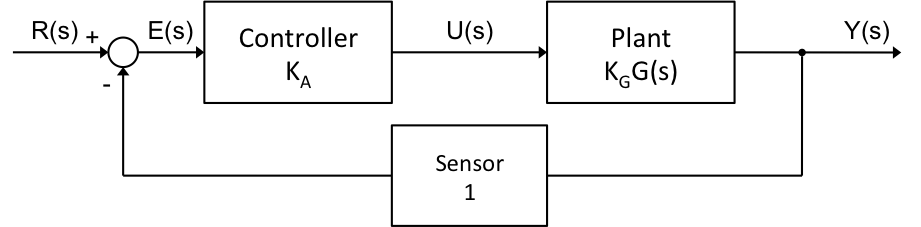
\includegraphics[width=1\linewidth]{closed_loop_diagram}
	\end{figure}
	The closed-loop transfer function is:
	\begin{center}
		$H(s) = \frac{Y(s)}{R(s)} = \frac{K_AK_GG(s)}{1 + K_AK_GG(s)}$.
	\end{center}
\end{frame}

\begin{frame}
\frametitle{Concept of the technique}
	Looking at this transfer function, we can conclude that the closed-loop roots depend on the amplifier gain $K_A$. We can now plot the locus of all possible roots of the characteristic equation: 
	\begin{equation}
		1 + K_AK_GG(s) = 0 \hspace{1em}
	\end{equation}
	as $K_A$ varies form $0$ to $\infty$. This results in a graph which can help us in selecting the best value of $K_A$.\\
	\vspace{1em}
	Furthermore, by studying the effects of additional poles and zeros, we can determine the consequences of additional dynamics in the loop. We can also extend this technique to examine the effect of other plant-parameter changes in order to achieve the best overall control design.
\end{frame}

\begin{frame}
\frametitle{Root Locus}
	\begin{block}{Definition I}
		The root locus is the set of values of s for which $1 + KG(s) = 0$ is statisfied as the real parameter $K$ varies from $0$ to $+\infty$. Often $G(s)$ is the open-loop transfer function of a system; in this case, roots on the locus are closed-loop poles of that system.
	\end{block}
	\begin{block}{Use of root loci}
		The root loci method provides a tool not only for selecting the gain but for designing the dynamic compensations as well.
	\end{block}
\end{frame}

\begin{frame}
\frametitle{Concept of the technique}
	For the further derivation, we assume that the system's open-loop transfer function $K_GG(s)$ is a rational function whose numerator is $K_Gb(s)$ and whose denominator is $a(s)$.$b(s)$ is a monic polynomial of degree $m$ and $a(s)$ is a monic polynomial of degree $n$ such that $n \geq m$.\\
	\vspace{1em}
	We assume the plant gain $K_G$ to be positive and define the root-locus parameter K as:
	\begin{center}
		$K = K_AK_G$
	\end{center}
\end{frame}

\begin{frame}
\frametitle{Concept of the technique}
\begin{block}{Root-Locus form}
	We can express Eq. (1) in different equivalent ways:
	\vspace{-1em}
	\begin{align*}
		1 + KG(s) &= 0,\\
		1 + K\frac{b(s)}{a(s)} &= 0,\\
		a(s) + Kb(s) &=0,\\
		G(s) & = -\frac{1}{K}.
	\end{align*}
\end{block}

\begin{alertblock}{Open-loop vs Closed-loop}
	The root-locus method can be thought of as a method for inferring properties of the closed-loop system given the open-loop transfer function $KG(s)$.
\end{alertblock}
\end{frame}

\begin{frame}
	\begin{example}
		\textbf{Problem}: a normalized transfer function of a DC motor is:
		\begin{equation}
		K_GG(s) = \frac{1}{s(s+1)}.
 		\end{equation}
 		Solve for the locus of roots with respect to $K_A$ of the closed-loop system created by feeding back the output as shown in the figure:
 		\begin{figure}
 			\centering
 			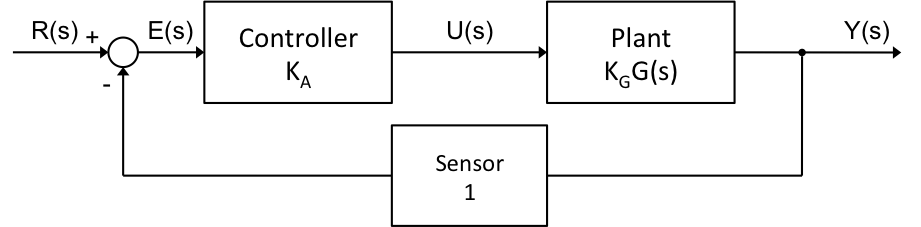
\includegraphics[width=0.8\linewidth]{closed_loop_diagram}
 		\end{figure}
 		Solve by using direct calculations of the root locations.
	\end{example}
\end{frame}

\begin{frame}
	\begin{exampleblock}{}
		\textbf{Solution}: in terms of our notation
		\vspace{-0.5em}
		\begin{columns}
			\begin{column}{0.2\textwidth}
				\begin{align*}
				m &=0,\\
				n &=2,
				\end{align*}
			\end{column}
			\begin{column}{0.2\textwidth}
				\begin{align*}
				K_G =1,\\
				K_A =K,
				\end{align*}
			\end{column}
			\begin{column}{0.2\textwidth}
				\begin{align*}
				b(s) =1,\\
				a(s) = 1.
				\end{align*}
			\end{column}
		\end{columns}
		\vspace{1em}
		We can use the root-locus form $a(s) + Kb(s) = 0$ to obtain a quadratic equation of which the roots will produce a graph.\\ 
		In this case, the quadratic equation:
		\begin{equation}
		s^2 + s + K = 0
		\end{equation}
		has roots:
		\begin{equation}
		r_1,r_2 = -\frac{1}{2} \pm \frac{\sqrt{1 - 4K}}{2}.
		\end{equation}
	\end{exampleblock}
\end{frame}

\begin{frame}
	\begin{exampleblock}{}
		The root locus is shown below
		\begin{figure}
			\centering
			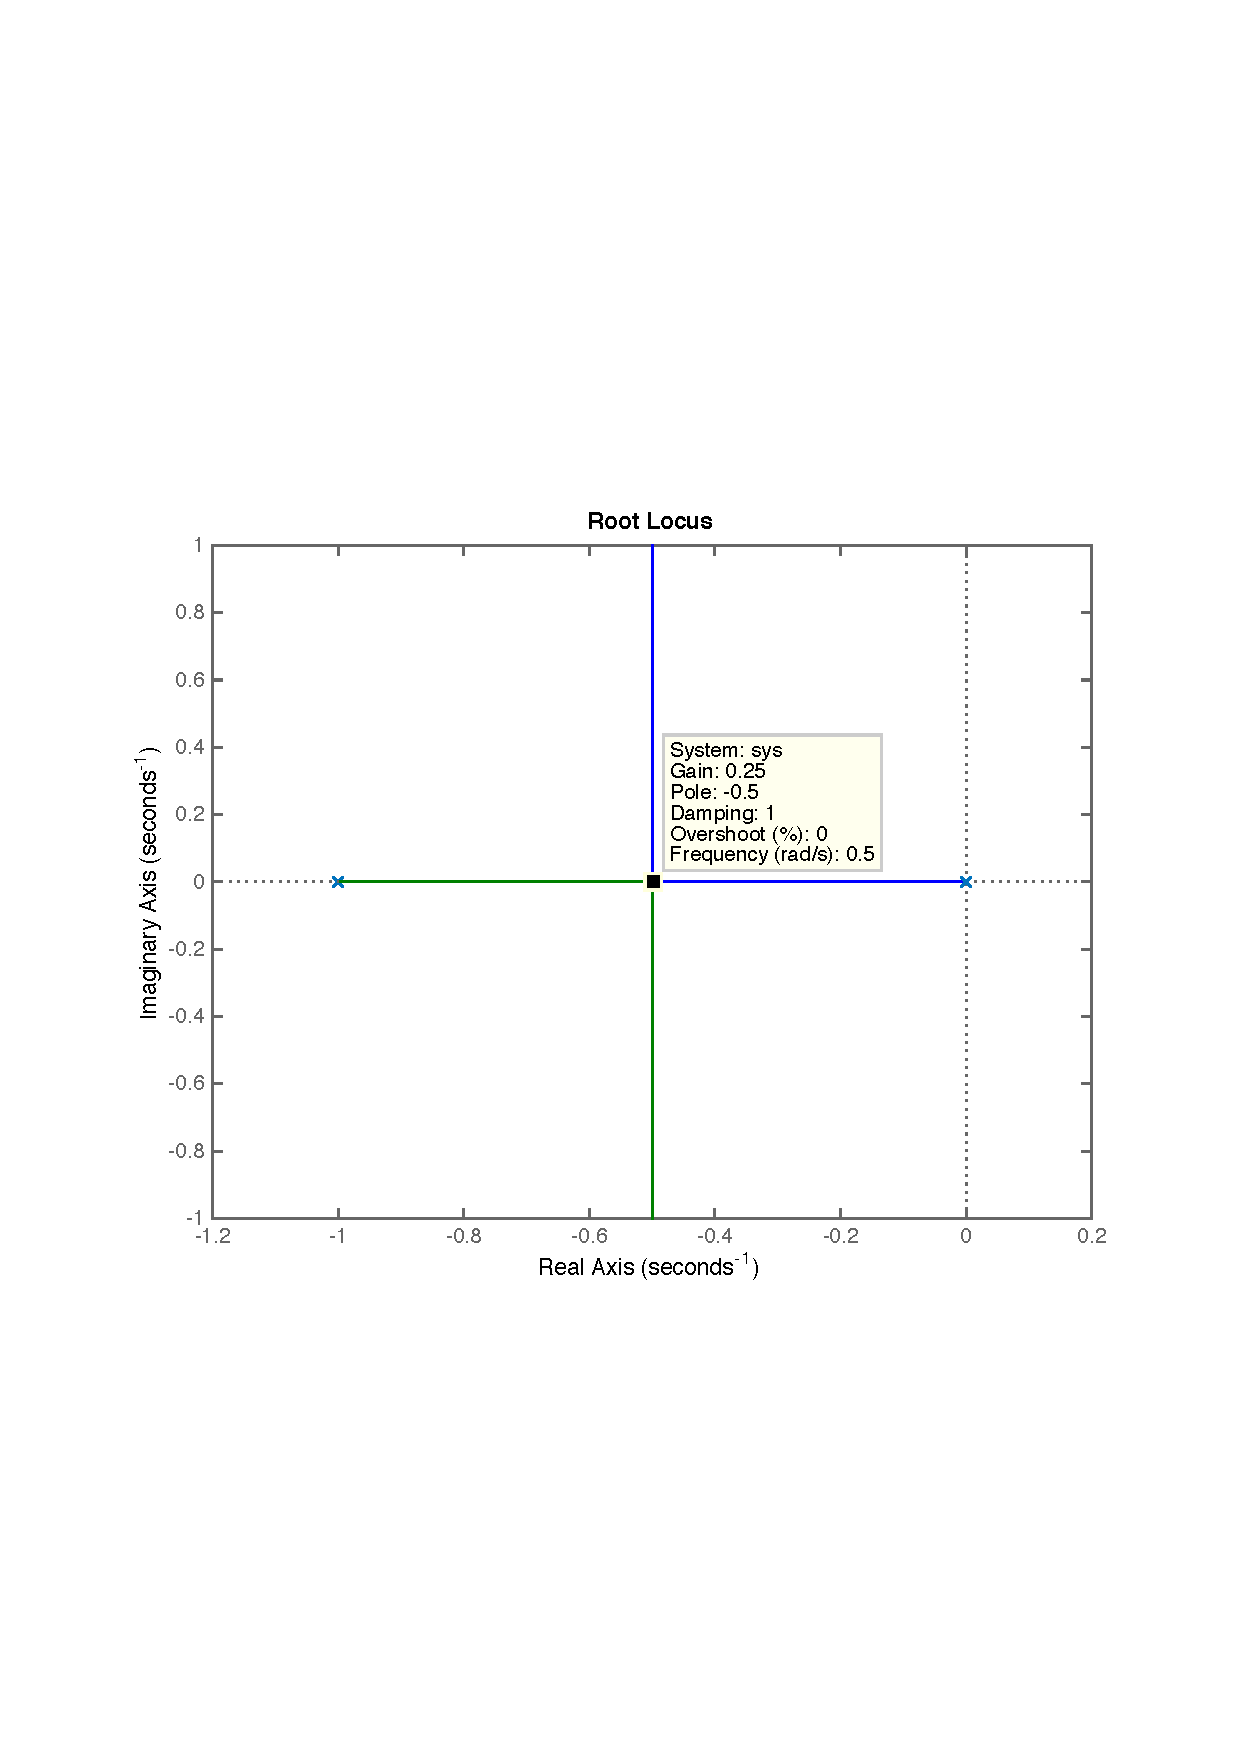
\includegraphics[width=0.7\linewidth]{root_locus_ex1}
		\end{figure}
	\end{exampleblock}
\end{frame}

\begin{frame}
	\begin{exampleblock}{}
		\begin{itemize}
		\item For $0\leq K \leq \frac{1}{4}$, the roots are real between $-1$ and $0$;
		\item At $K = \frac{1}{4}$ there are two roots at $-\frac{1}{2}$;
		\item For $K>\frac{1}{4}$ the roots become complex, with a real part of $-\frac{1}{2}$ and an imaginary part that increases essentially in proportion to the square root of K
		\end{itemize}
		\vspace{1em}
		We can now compute K at the point where the locus crosses $\zeta = 0.5$: we know that if $\zeta = 0.5$, then $\theta = 30^{\circ}$ and the magnitude of the imaginary part of the root is $\sqrt{3}$ times the magnitude of the real part. The magnitude of the real part is $\frac{1}{2}$ and thus, we have: \begin{equation}
		\frac{\sqrt{4K - 1}}{2} = \frac{\sqrt{3}}{2}
		\end{equation}
		and therefor, $K = 1$.
		\end{exampleblock}
\end{frame}

\section{How To Draw Root Loci}

\subsection{General Approach}

\begin{frame}
\frametitle{General approach}
	Now look at the equation: $G(s) = -\frac{1}{K}$. If $K$ is to be real and positive, $G(s)$ must be real and negative. This means that if we arrange G(s) in polar form as magnitude and phase, $G(s)$ must have the opposite phase of $K$ in order to satisfy the equation above. We can thus define a root locus in terms of this phase condition:  
	\vspace{0.5em}
	\begin{block}{Definition II}
		The root locus of $G(s)$ is the set of points in the s-plane where the phase of $G(s)$ is $180^{\circ}$.	
	\end{block}
	
\end{frame}

\begin{frame}
\frametitle{General approach}
	Since the phase remains unchanged if an integral multiple of $360^{\circ}$ is added, we can express Definition 2 as: $\angle G(s) = 180^{\circ} + 360^{\circ}$, where $l$ is any integer. While it is very difficult to solve a high-order polynomial, computing the phase is relatively easy.\\
	\vspace{1em}
	The usual case is when $K$ is real and positive; we call this case the \textbf{positive or $180^{\circ}$ locus}. When $K$ is real and negative, $G(s)$ must be real and positive of $s$ to be on the locus. Therefor, the phase of $G(s)$ must be $0^{\circ}$. This special case is called a \textbf{negative or $0^{\circ}$ locus}.\\
	\vspace{1em}
	Measuring the phase is easy but measuring the phase at every point in the $s$-plane is hardly practical. It would be better if there would exist some general guidelines we can use for determining where the root locus is.
\end{frame}

\begin{frame}
\frametitle{Overview of the guidelines}
	Drawing the root loci yourself can be done by following the next steps:
	\vspace{0.5em}
	\begin{enumerate}
		\item Mark poles with $\times$ and zeros with $\circ$;
		\item Draw the locus on the real axis to the left of an odd number of real poles plus zeros;
		\item Draw the asymptotes, centered at $\alpha$ and leaving at angles $\phi_l$, where:
		\vspace{-0.5em}
		\begin{align*}
			n - m &= $ number of asymptotes$\\
			\alpha &= \frac{\varSigma p_i - \varSigma z_i}{n-m}\\
			\phi_l &= \frac{180^{\circ} + 360^{\circ}(l - 1)}{n - m}, l = 1,2,...,n-m.
		\end{align*}
	\end{enumerate}
\end{frame}

\begin{frame}
\frametitle{Overview of the guidelines}
	\begin{enumerate}
	\setcounter{enumi}{3}
	\item Compute locus departure angles from te poles and arrival angles at the zeros:
	\begin{align*}
	q\phi_{dep} &= \varSigma\psi_i - \varSigma\phi_i - 180^{\circ} - 360^{\circ}l,\\
	q\psi_{arr} &= \varSigma\phi_i - \varSigma\psi_i + 180^{\circ} + 360^{\circ}l,
	\end{align*}
	where $q$ is the order of the pole or zero and $l$ takes on $q$ integer values so that the angles are between $\pm180^{\circ}$. $\Sigma \phi_i$ is the sum of the angles of the (remaining) poles and $\Sigma \psi_i$ is the sum of the angles of the (remaining) zeros.
	
	\end{enumerate}
\end{frame}

\begin{frame}
\frametitle{Overview of the guidelines}
	\begin{enumerate}
	\setcounter{enumi}{4}
	\item If further refinement is required at the stability boundary: Assume $s_0 = j\omega_0$ and compute the point(s) where the locus crosses the imaginary axis for positive values of $K$, and/or use Routh's stability criterion. (This step may not be necessary).
	\item Use the results from the study of multiple roots to help in sketching how locus segments come together and break away: two segments come together at $180^{\circ}$ and break away at $\pm 90^{\circ}$, three locus segments approach each other at relative angles of $120^{\circ}$ and depart at angles rotated by $60^{\circ}$.
	\item Complete the locus, using the facts developed in the previous steps and making reference to the illustrative loci for guidance. The locus branches start at poles and at zeros or infinity.
	\end{enumerate}
\end{frame}

\begin{frame}
\frametitle{Guidelines in practice}
	\begin{block}{ }
		We will now apply the guidelines on an example transfer function, to indicate how the guidelines must be used.\\
		\vspace{0.5em}
		Transfer function:
		\vspace{-0.5em}
		\begin{equation}
		G(s) = \frac{1}{s[(s+4)^{2} + 16]}
		\vspace{-0.5em}
		\end{equation}
		Using Definition II, we can check whether a point $s_0$ lies on the root locus for some value of $K$ by checking if the following expression is valid: 
		\vspace{-0.5em}
		\begin{equation}
		\angle 1 - \angle s_0 -\angle [(s_0 + 4)^2 + 16] = 180^{\circ} + 360^{\circ}l
		\vspace{-0.5em}
		\end{equation}
		but as already mentioned, it is not practical to do this for every point $\rightarrow$ we will use the general guidelines. 
	\end{block}
\end{frame}	

\begin{frame}
\frametitle{Guidelines in practice}
	\begin{block}{STEP 1: the open-loop $\times's$ and $\circ's$}
		\begin{figure}
			\centering
			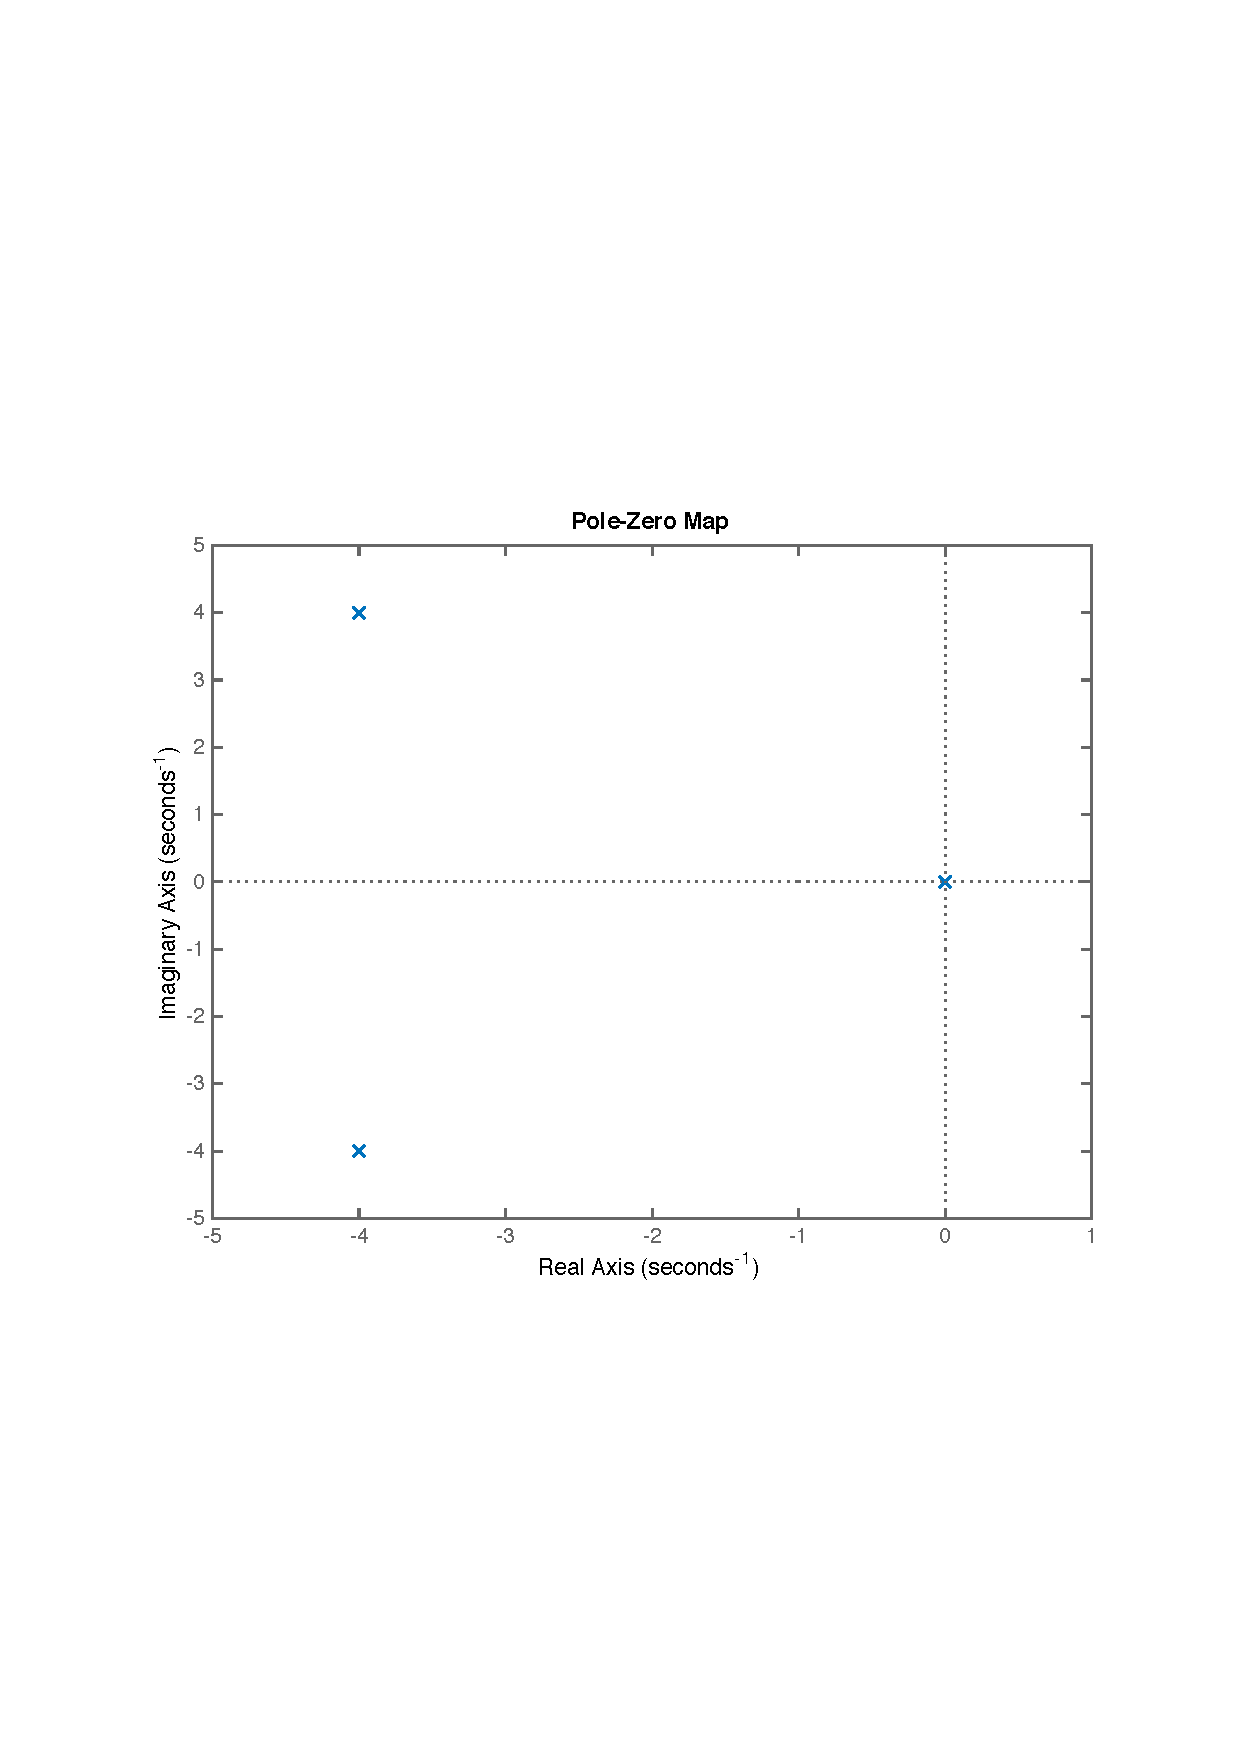
\includegraphics[width=0.6\linewidth]{how_to_draw_ex1}
		\end{figure}
	\end{block}
\end{frame}

\begin{frame}
\frametitle{Guidelines in practice}
	\begin{block}{STEP 2: locus on real axis}
		The portion of the real axis to the left of an odd number (counted from the right) of open loop poles and zeros are part of the loci:
		\vspace{-0.5em}
		\begin{figure}
			\centering
			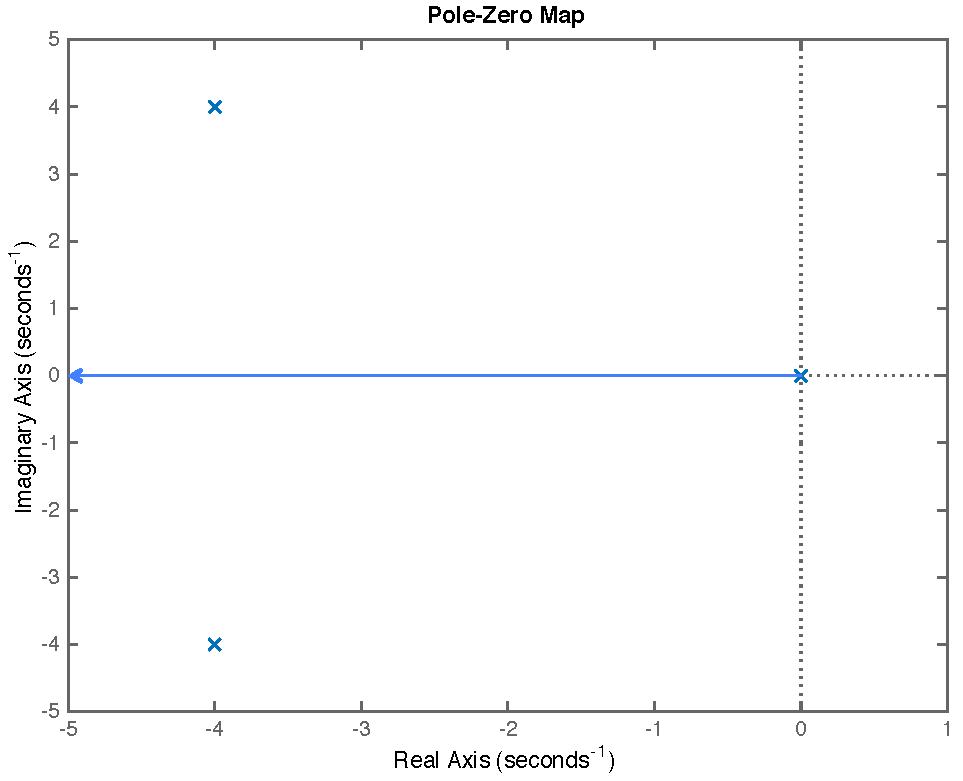
\includegraphics[width=0.6\linewidth]{how_to_draw_ex2}
		\end{figure}
	\end{block}
\end{frame}

\begin{frame}
\frametitle{Guidelines in practice}
	\begin{block}{STEP 3: asymptotes for large values of K}
		As K approaches $\infty$, the equation $G(s) = -\frac{1}{K}$ can be satisfied only if $G(s) = 0$ where $G(s) = \frac{b(s)}{a(s)}$.\\
		\vspace{1em}
		We can now substitute this in $1 + KG(s) = 0$, resulting in following equation:
		\begin{equation}
		1 + K\frac{b(s)}{a(s)} = 1 + K\frac{s^m + b_1s^{m-1} + ... + b_m}{s^n + a_1s^{n-1} + ... + a_n} = 0
		\end{equation}
		Since $n < m$, $G(s) = 0$ can occur when: 
	\begin{itemize}
			\item $b(s) = 0$;
			\item $s \rightarrow \infty$.
		\end{itemize}
	\end{block}
\end{frame}

\begin{frame}
\frametitle{Guidelines in practice}
	\begin{block}{STEP 3: asymptotes for large values of K}
		We now look closer to the second condition: $G(s) = 0$ when $s \rightarrow \infty$.\\
		\vspace{1em}
		For very large values of $s$, the highest-order power of $s$ in Eq.(8) predominates. We can divide $a(s)$ by $b(s)$ and match the dominant two terms (highest powers in s) to the expansion $(s-\alpha)^{n-m}$, resulting in the following approximation:
		\begin{equation}
			1 + K\frac{1}{(s-\alpha)^{n-m}}
		\end{equation}
		We need to find the locus for the asymptotic system (Eq.(8)) and $\alpha$.
	\end{block}
\end{frame}

\begin{frame}
	\frametitle{Guidelines in practice}
	\begin{block}{STEP 3: asymptotes for large values of K}
		To find the locus, we choose $s_0 = Re^{j\phi}$ for some large value of $R$ and some variable $\phi$.\\
		\vspace{1em}
		Since all poles of Eq.(9) are in the same place, the angle of its transfer function is $180^{\circ}$ if all $n-m$ angles, each equal to $\phi_l$, sum to $180^{\circ}$. Therefor, $\phi_l$ is given by: 
		\begin{equation}
		\phi_l = \frac{180^{\circ} + 360^{\circ}l}{n-m}, l = 1,2,...,n-m
		\end{equation}
		For our system: $n-m=3$, thus $\phi_1, \phi_2, \phi_3 = 60^{\circ}, 180^{\circ}, 300^{\circ}$.
		All the lines of the asymptotic locus come from $s_0 = \alpha$.
	\end{block}
\end{frame}

\begin{frame}
	\frametitle{Guidelines in practice}
	\begin{block}{STEP 3: asymptotes for large values of K}
		To determine $\alpha$ we use a simple property of polynomials. Suppose we have a monic polynomial with coefficients $a_i$ and roots $p_i$ and we equate the polynomial form with the factored form:
		\begin{center}
			$s^n + a_1s^{n-1} + a_2s^{n-2} + ... + a_n = (s-p_1)(s-p_2)...(s-p_n).$
		\end{center}
		If we multiply out the factors on the right side of this equation, we can see that the coefficient of $s^{n-1}$ is $-p_1 - p_2 - ... - p_n$. On the left side of the equation we see that this term is $a_1$.\\
		\vspace{1em}
		Consequently $a_1 = -\Sigma p_i$, the coefficient of the second-highest term in a monic polynomial is the negative sum of its roots (the poles of $G(s)$). The same can be concluded for $b_1 = -\Sigma z_i$.
	\end{block}
\end{frame}

\begin{frame}
	\frametitle{Guidelines in practice}
	\begin{block}{STEP 3: asymptotes for large values of K}
		Applying these results in the closed-loop characteristic polynomial, leads to:
		\begin{center}
			$s^n + a_1 s^{n-1} + ... + a_n + K(s^m + b_1 s^{m-1} + ... + b_m) = 0$.
		\end{center}
		The negative of the sum of the poles is the coefficient of $s^{n-1}$ and is independent of $K$ if $m < n-1$. However, since this is the closed-loop characteristic equation, this coefficient is the negative of the sum of the roots of the closed-loop system $\Sigma r_i$, hence
		\begin{itemize}
			\item the center point of the roots does not change with $K$ if $m < n-1$;
			\item $-\Sigma r_i = -\Sigma p_i$.
		\end{itemize}
		\end{block}
\end{frame}

\begin{frame}
	\frametitle{Guidelines in practice}
	\begin{block}{STEP 3: asymptotes for large values of K}
		For large values of $K$, $m$ of the roots $r_i$ are approximately equal to the zeros $z_i$ and $n-m$ of the roots are from the asymptotic $\frac{1}{(s-\alpha)^{n-m}}$ system, whose poles add up to $(n-m)\alpha$. Combining these results we conclude that the sum of all the roots equals the sum of those roots that go to infinity plus the sum of those roots that go to the zeros of $G(s)$:
		\begin{center}
			$+\Sigma r_i = + (n-m)\alpha + \Sigma z_i = +\Sigma p_i$.
		\end{center}
		Solving for $\alpha$ we get 
		\begin{center}
			$\alpha = \frac{\Sigma p_i - \Sigma z_i}{n-m}$.
		\end{center}
	\end{block}
\end{frame}

\begin{frame}
	\frametitle{Guidelines in practice}
	\begin{block}{STEP 3: asymptotes for large values of K}
		Complex poles and zeros always occur in complex conjugate pairs, consequently in the sums $\Sigma p_i$ and $\Sigma z_i$ the imaginary parts will always add to zero.\\
		\vspace{1em}
		For our system: $\alpha = \frac{-4-4+0}{3-0} = -2.67.$\\
		\vspace{1em}
		We can now use the results for $\phi_1, \phi_2, \phi_3 and \alpha$ to draw the asymptotes. 
	\end{block}
\end{frame}

\begin{frame}
\frametitle{Guidelines in practice}
	\begin{block}{STEP 3: asymptotes for large values of K}
		Resulting in the following figure
		\vspace{-0.5em}
		\begin{figure}
			\centering
			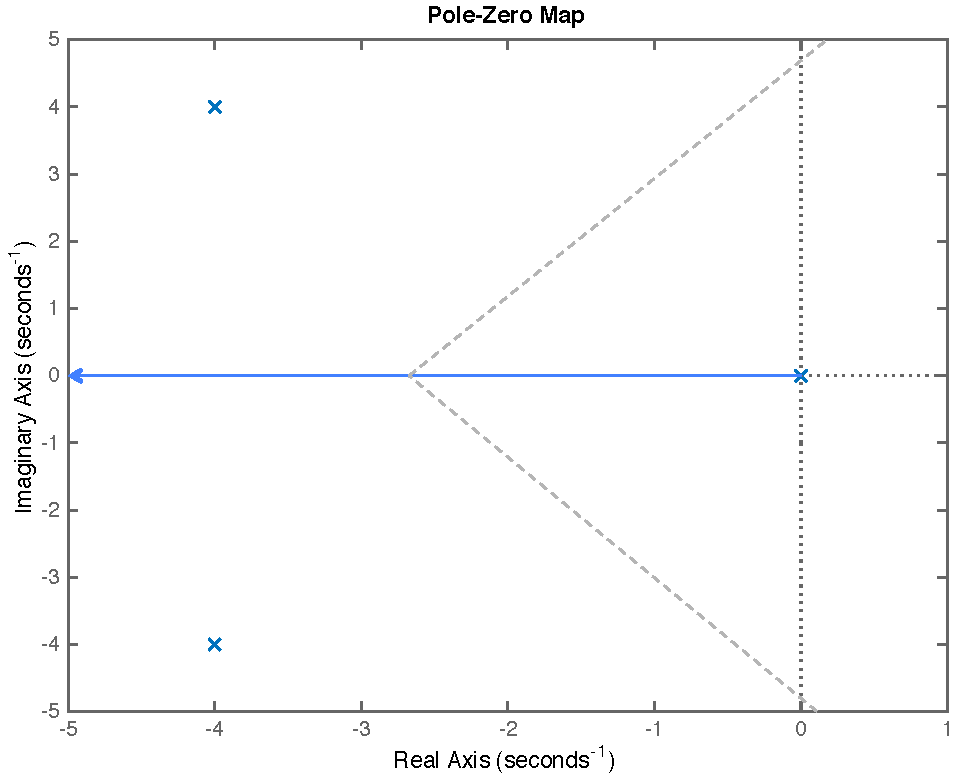
\includegraphics[width=0.6\linewidth]{how_to_draw_ex3}
		\end{figure}
	\end{block}
\end{frame}

\begin{frame}
	\frametitle{Guidelines in practice}
	\begin{block}{STEP 4: departure and arrival angles}
		We know that the locus begins at the $\times's$ and that it goes to either $\circ's$ or to infinity along the radial asymptotic lines.\\
		\vspace{1em}
		We next compute the angle by which a branch of the locus departs from one of the poles. We take a test point $s_0$ very near pole 2 at $-4+4j$ and compute the angle of $G(s_0)$ (illustration see next slide). We select the test point close enough to pole 2 that the angles $\phi_1$ and $\phi_3$ to the test point can be considered the same as those angles to pole 2: $\phi_1 = 90^{\circ}$ and $\phi_3 = 135^{\circ}$. 
	\end{block}
\end{frame}

\begin{frame}
	\frametitle{Guidelines in practice}
	\begin{block}{STEP 4: departure and arrival angles}
		\begin{figure}
			\centering
			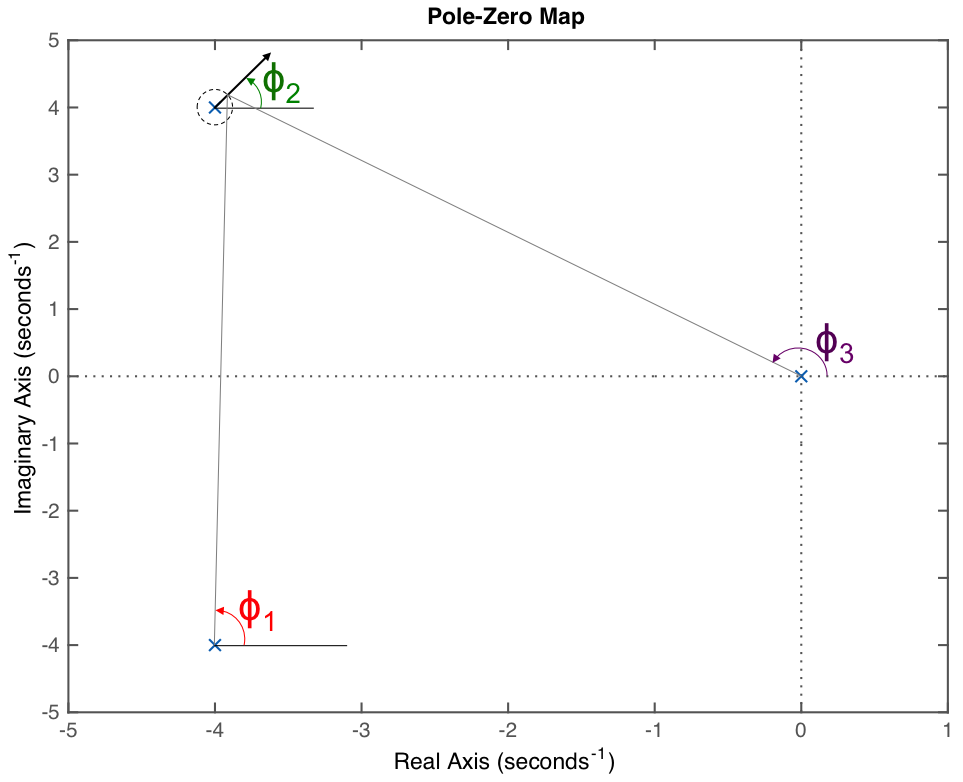
\includegraphics[width=0.6\linewidth]{how_to_draw_ex4}
		\end{figure}
	\end{block}
\end{frame}

\begin{frame}
\frametitle{Guidelines in practice}	
	\begin{block}{STEP 4: departure and arrival angles}
		We can calculate $\phi_2$ from the angle condition:
		\begin{center}
			$-90^{\circ} - \phi_2 - 135^{\circ} = +180^{\circ} + 360^{\circ}l$
		\end{center}
		where $l$ is chosen so that $-180^{\circ} < \phi_2 < +180^{\circ}$. If we take $l = -1$, then $\phi_2 = -45^{\circ}$.\\
		\vspace{1em}
		By the complex conjugate symmetry of the plots, the angle of departure of the locus near pole 1 at $-4 - 4j$ will be $+45^{\circ}$. The angle of departure from pole 3 at the origin is $180^{\circ}$.
	\end{block}
\end{frame}

\begin{frame}
\frametitle{Guidelines in practice}	
	\begin{block}{STEP 5: Estimate the points of the locus on the imaginary axis}
		We will not discuss this since it is not always necessary and it becomes very difficult for fourth- or higher-order systems.
	\end{block}
	
	\begin{block}{STEP 6: Estimate the location of multiple roots and determine their arrival and departure angles}
		
	\end{block}
\end{frame}

\subsection{Rules of thumb for a quick drawing}

\begin{frame}
	INCLUDE SLIDES FROM PREVIOUS PRESENTATION
\end{frame}

\section{Root Loci and MATLAB}

\begin{frame}
	INCLUDE SLIDES WITH MATLAB EXAMPLES
\end{frame}